\chapter{Projeto e Implementação}\label{chp:ml}


\section{Tratamento dos dados}\label{sec:data1}

\subsection{Dados obtidos do Repositório UCI}
	Para grande parte dos testes de \textit{cross-validation}, foi usado o \textit{dataset}  \textit{UJIIndoorLoc} apresentado em \cite{uji}. O \textit{dataset} consiste em diversas medidas de potência de sinal \textit{Wi-fi} medidas com diversos aparelhos celulares em 3 prédios diferentes de uma faculdade. As medidas estão separadas por prédio, andar e sala. Para os fins dessa monografia, serão realizados testes com medidas sempre de um mesmo andar, afim de classificar as zonas de um mesmo ambiente.  Esse  \textit{dataset} usa a constante $100$ para designar valores não medidos. Para começar o tratamento os substituímos pelo valor de $-120$ (dB), que para todos os fins práticos, é uma medida de potência que representa um valor nulo, já que representa um valor de potência insignificante. E finalmente, antes de serem usados para treinar os modelos, os dados são transformados de modo a ficarem com média 0 e variância 1 por coluna, o que é necessário para evitar comportamentos indesejados dos algoritmos de ML.

A transformação é realizada da seguinte maneira, com $X_j$ representando a j-ésima coluna da matriz de dados, com média $\mu$ e desvio-padrão $\sigma$, para cada elemento $i$ dessa coluna:

\begin{center}
$X_{ij}=\frac{X_{ij}-\mu}{\sigma}$
\end{center}

\subsection{Dados do Servidor}

De modo análogo aos dados pegos do Repositório UCI, a matriz de dados é transformada para ter média nula e variância unitária em cada coluna, sendo que antes disso valores nulos são substituídos por $-120$.




\section{Formato dos dados tratados}
A matriz de dados, depois de tratada, tem o seguinte formato:

\begin{center}
\begin{blockarray}{cccccc}
$ZoneID$ & $BSSID_1$ & $BSSID_2$ & ... &  $BSSID_n$ \\
\begin{block}{(ccccc)c}
  1&-70 & -92 &   ... &-87&  $ Measure_1$ \\
  2&-89 & -80 & ... & -63&    $Measure_2 $\\
  3&-28 & -120 & ...&   -35& $Measure_3$ \\
   \vdots& \vdots &  \vdots & $\ddots$ &  \vdots &    \vdots \\
  1&-48 & -36 & ... &   -29&  $Measure_n$ \\
\end{block}
\end{blockarray}
\end{center}

Cada coluna representa a medida de uma \textit{BSSID} (i.e. um Roteador), ou seja, uma \textit{feature} para o ML, e cada linha é um ponto de treino (i.e.  uma medida para cada  \textit{BSSID}, nossas \textit{features}).


\section{Modelos Usados e \textit{Cross-Validation} de parâmetros }

A chamada \textit{cross-validation} dos modelos de ML é o teste para encontrar os parâmetros ótimos para o treinamento. Um dos métodos escolhidos de \textit{cross-validation} foi o \textit{k-fold}. O método \textit{k-fold} divide o dataset em $K$ subconjuntos de igual tamanho e então um dos conjuntos é usado como validação do treinamento feito pelos $K-1$ subconjuntos restantes. O processo é repetido $K$ vezes e em cada subdivisão possível podem ser usados valores de parâmetros de treino distintos. Para a comparação dos modelos, serão feitos diversos testes com um número crescente de zonas de classificação. Nesse caso, são escolhidas iterativamente e aleatoriamente $n$ zonas do \textit{dataset}  \textit{UJIIndoorLoc}, são pegos todos os pontos associados as $n$ zonas selecionadas. Então, o \textit{dataset}  é separado em 80\% de pontos de treino e 20\% para testes. Para valores de $n$ de 1 a 30 são finalmente medidos as taxas de erro de cada algoritmo e essa informação é apresentada em gráficos.

\subsection{KNN : K-Nearest-Neighbors }


Para o algoritmo de KNN, foram feitos dois testes de \textit{cross-validation}. No primeiro, a métrica de distância foi decidida, e no segundo, o número de vizinhos ($K$).
Para que fosse definida a métrica de distância, foi usado o método  \textit{k-fold}  com $K=2$. E em cada \textit{fold} o modelo foi treinado com uma métrica diferente. Foram calculados 20 conjuntos diferentes de \textit{folds} e foi tirada a média do erro de validação para cada uma das métricas.


\begin{figure}[H]
\centering
\caption{Erros para uso de Diferentes Distâncias}
 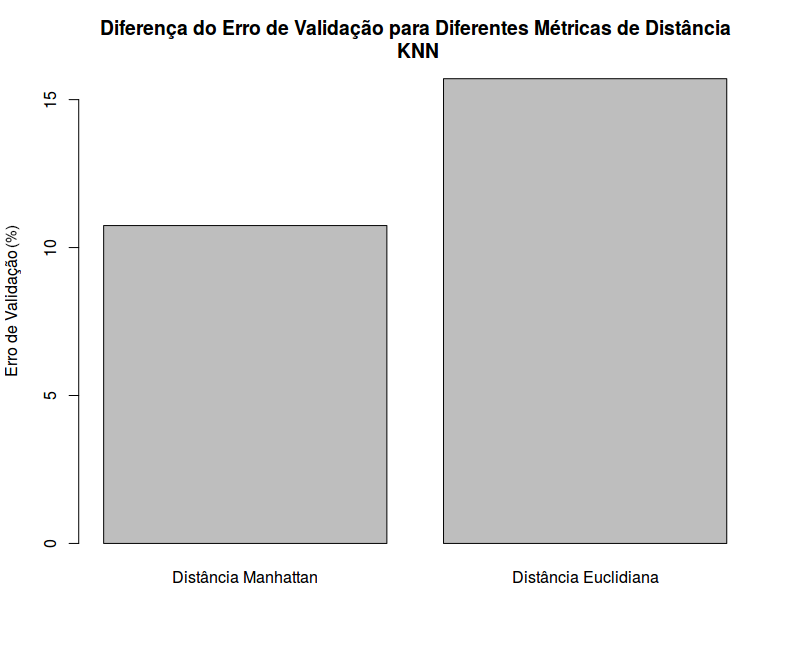
\includegraphics[width=0.9\textwidth]{euclidianManhattanknn21zonas}
\label{fig:euclidian}
\end{figure}


Depois, foi usado o método  \textit{k-fold} com $K=10$ para a decisão do número de vizinhos. Foram testados os valores de 1 até 10 para o número de vizinhos. Na imagem a seguir vemos detalhes desse teste.


\begin{figure}[H]
\centering
\caption{Erro em função do número de vizinhos}
 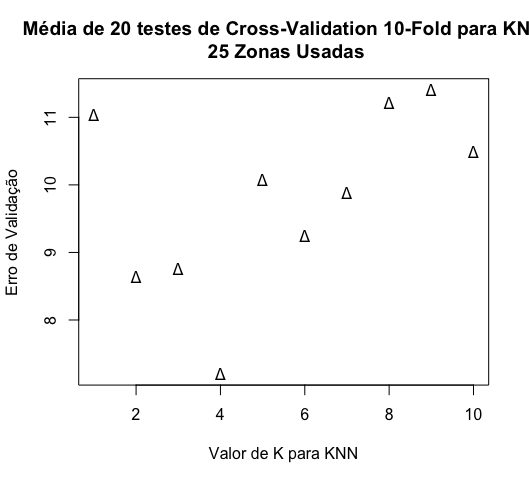
\includegraphics[width=0.9\textwidth]{CrossValKNN25zonasvalorK}
\label{fig:crossValKNN}
\end{figure}



Podemos concluir então que (1) o erro é menor no geral com a distância de \textit{Manhattan} e (2) embora tenha muita variância envolvida no teste, o valor de K que minimiza o erro fica proximo de 4 vizinhos.


No restante do trabalho foi escolhido o valor de $K=4$ vizinhos.



\subsection{Rede Neural}

Para a \textit{cross-validation} das Redes Neurais, também foi usado o método de  \textit{k-fold} com $K=10$. Para cada uns dos\textit{folds} foi testado um número de neurônios em uma  \textit{hidden-layer} única. (Outros testes mostraram não valer a pena para o nosso problema usar mais de uma camada de  \textit{hidden layer} ou \textit{deep learning}). Os resultados são mostrados a seguir:



\begin{figure}[H]
	\centering
	\caption{Erro para diversas quantidades de neurônios na rede neural.}
  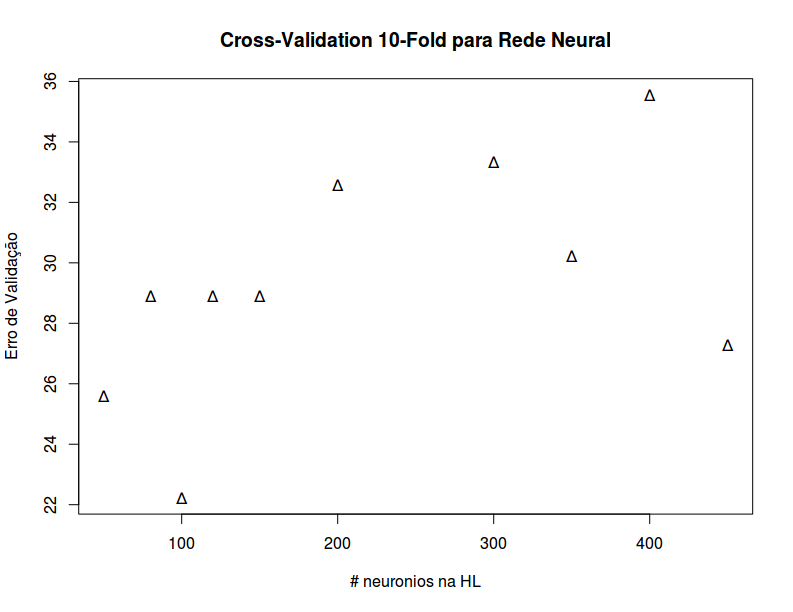
\includegraphics[width=0.9\textwidth]{CROSSVALE4ZonasNNCERTO}
\label{fig:crossNN}

\end{figure}




Concluímos que o número ideal de neurônios na  \textit{hidden-layer} está próximo de 200. Porém, com estudos e testes mais detalhados ficou claro que as Redes Neurais não são ideias para o nosso projeto, por não conseguirem capturar de forma satisfatória o modelo do nosso problema. Além disso, o algoritmo de \textit{back propagation} se mostra muito mais custoso em relação a memória e processamento se comparado aos outros algoritmos usados no projeto, demorando cerca de 10 vezes mais para o treinamento que todos os outros modelos juntos. Portanto, seu uso foi descartado.

\subsection{Arvore de decisão}


Baseado no trabalho apresentado por \cite{comparative}, foi escolhida uma implementação do algoritmo C4.5 \cite{quinlan} em Java, da biblioteca Weka, para serem geradas árvores de decisão. Os métodos porém foram chamados pela interface da Weka para R, chamada RWeka.
A função J48 do Weka foi testada com o os pontos de treino referentes ao primeiro andar do prédio 1 (i.e. BuildingID 1, FloorID 0)  do dataset \textit{UJIIndoorLoc}. Foi levantada a curva de erro de classificação para uma quantidade crescente de pontos de treino (como explicado em 2.3).


\begin{figure}[H]
\centering
\caption{Teste de Validação do Algoritmo C4.5}
 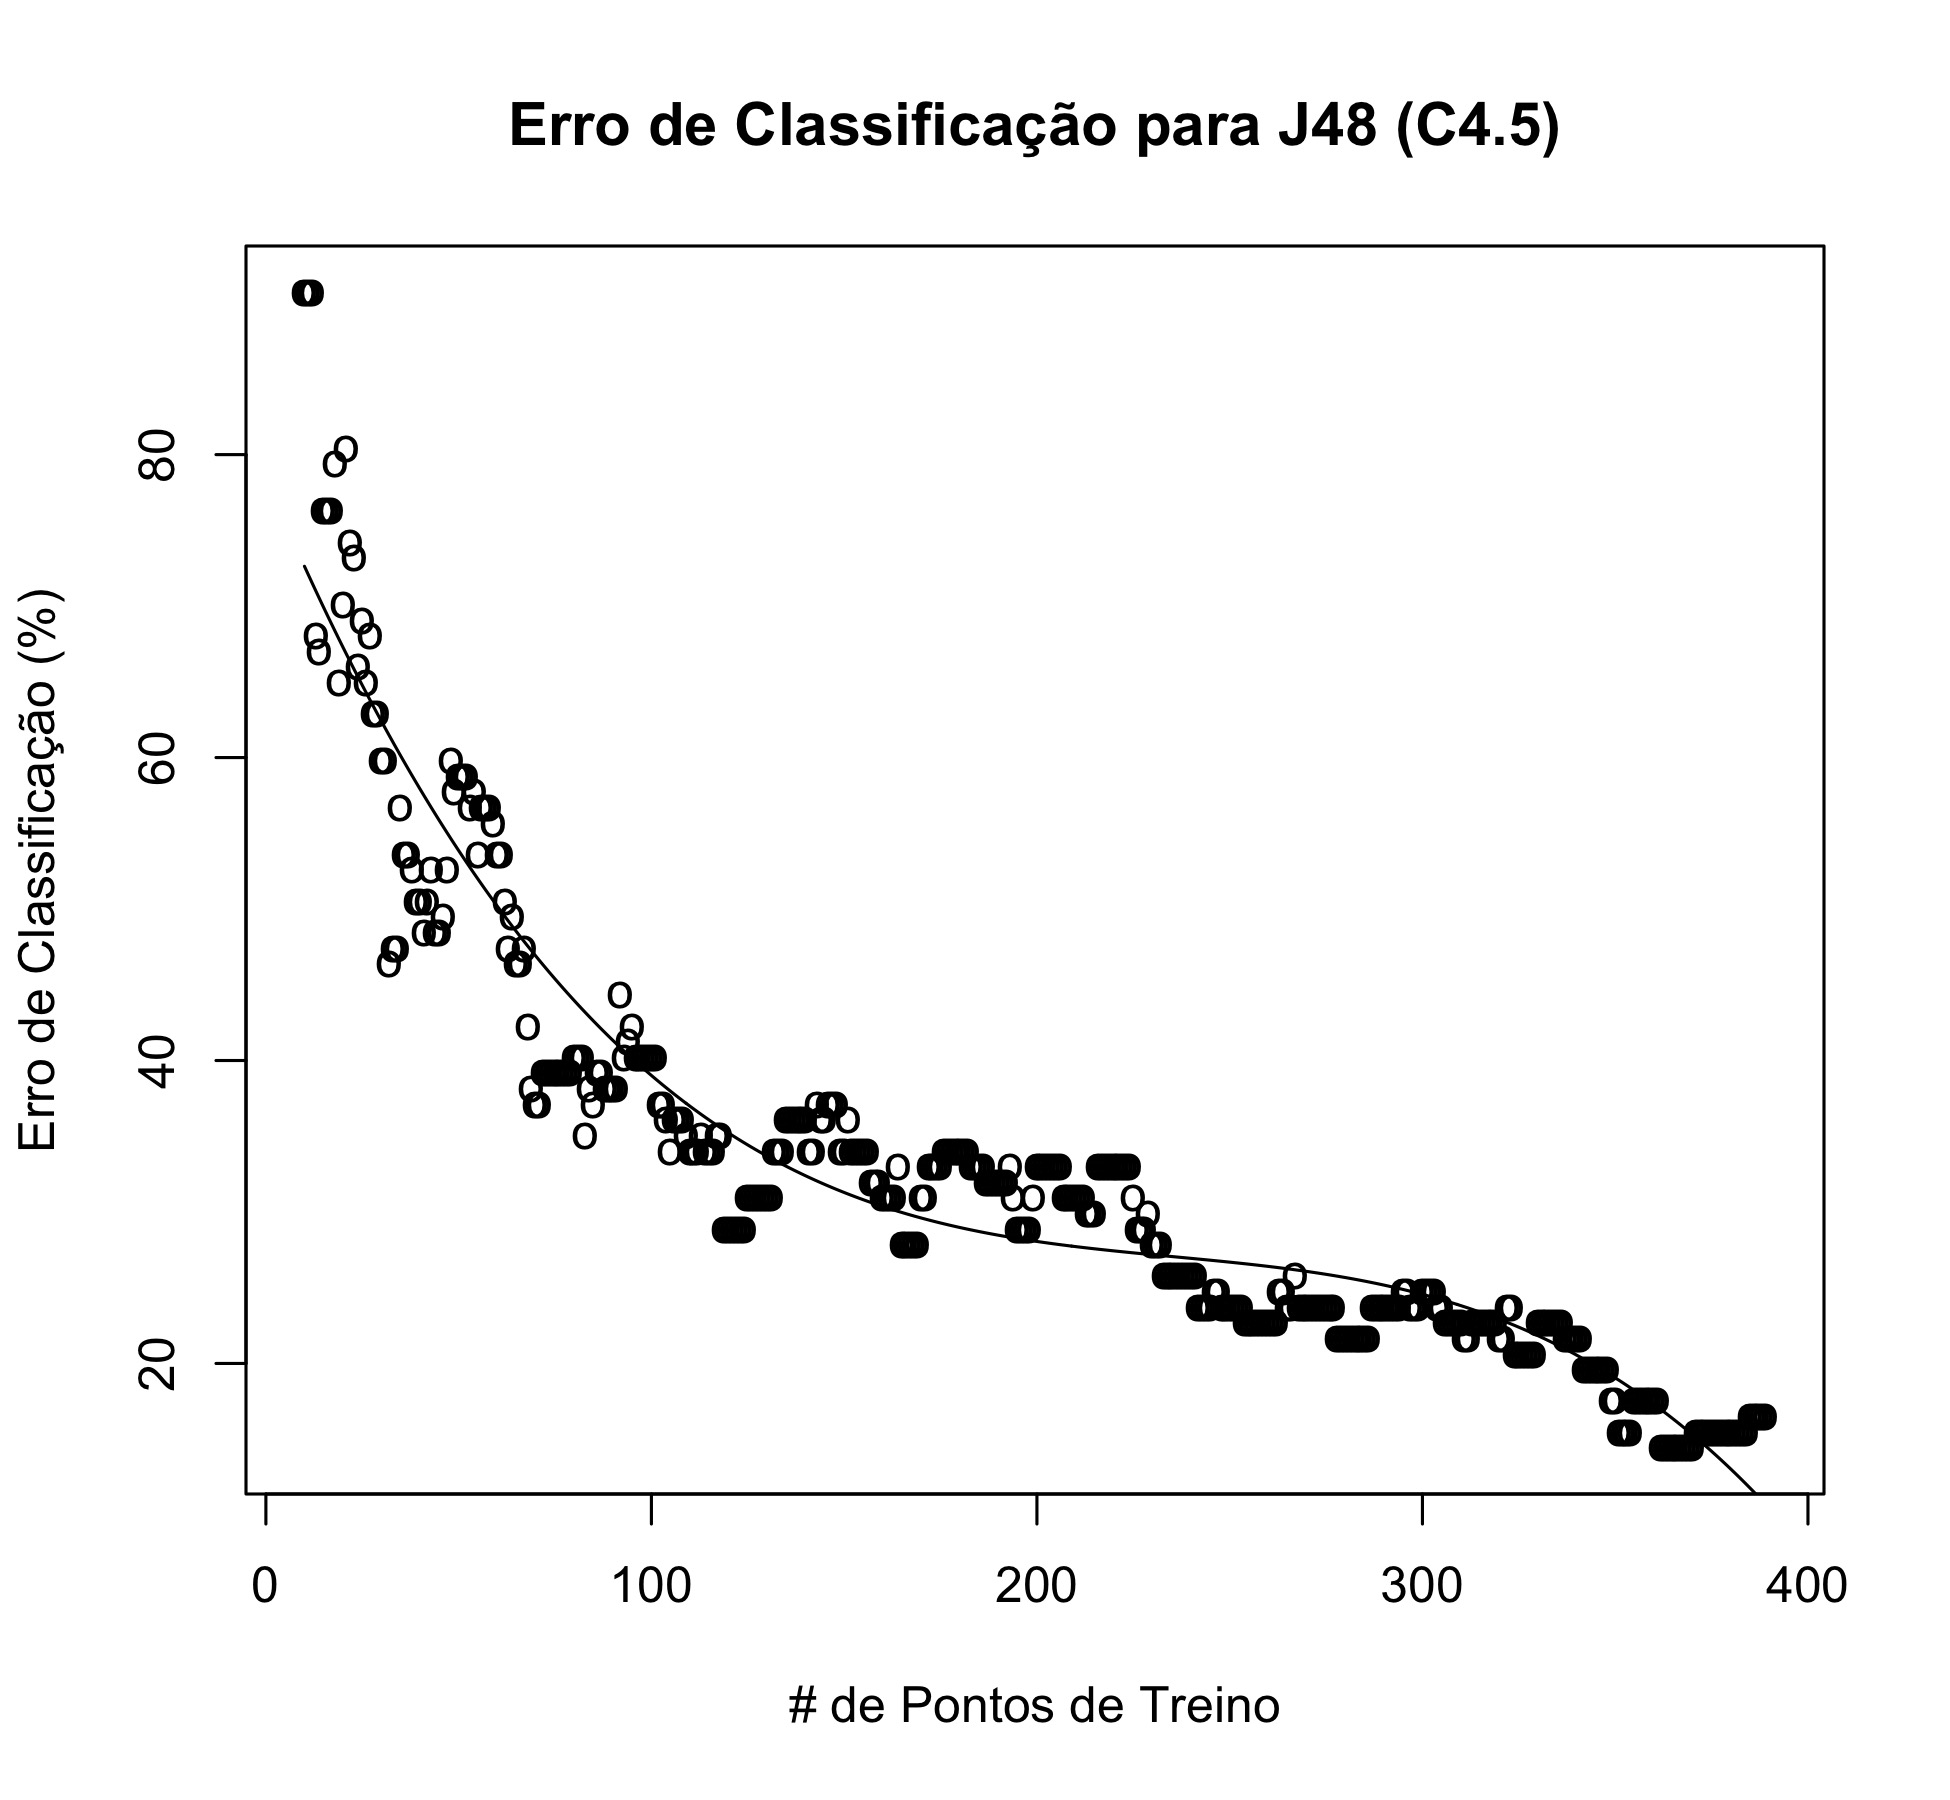
\includegraphics[width=0.9\textwidth]{J48Validacaopredio1andar0}
\label{fig:validationC4.5}
\end{figure}

\subsubsection{Acoplamento com o Algoritmo AdaBoost}




\textit{Boosting} é a ideia em ML de criar uma predição forte e precisa combinando diversas previsões mais fracas. O algoritmo AdaBoost \cite{adaboost} é um método para melhorar a precisão de classificadores fracos (i.e. \textit{Weak Learners}) por meio de uma votação ponderada que leva em conta o erro de diversos votadores fracos treinados no processo. É provado que o modelo final se torna um classificador forte \cite{explainingadaboost}. Por definição, um classificador fraco é aquele que consistentemente consegue ser melhor que um chute para a classificação (e.g. o erro é menor que 50\% para o caso de duas classes possíveis de classificação).

Também baseados em \cite{comparative} e \cite{comparativeEN}. Usaremos o algoritmo AdaBoost  e sua implementação na biblioteca Weka para melhorar a precisão das árvores de decisão C4.5. A seguir vemos um gráfico comparando a classificação para o mesmo andar do \textit{dataset UJIIndoorLoc} com os mesmos pontos de teste e uma quantidade crescente de pontos de treino, assim como feito no tópico anterior.


\begin{figure}[!h]
\centering
\caption{Comparação do C4.5 com o uso do AdaBoost}
 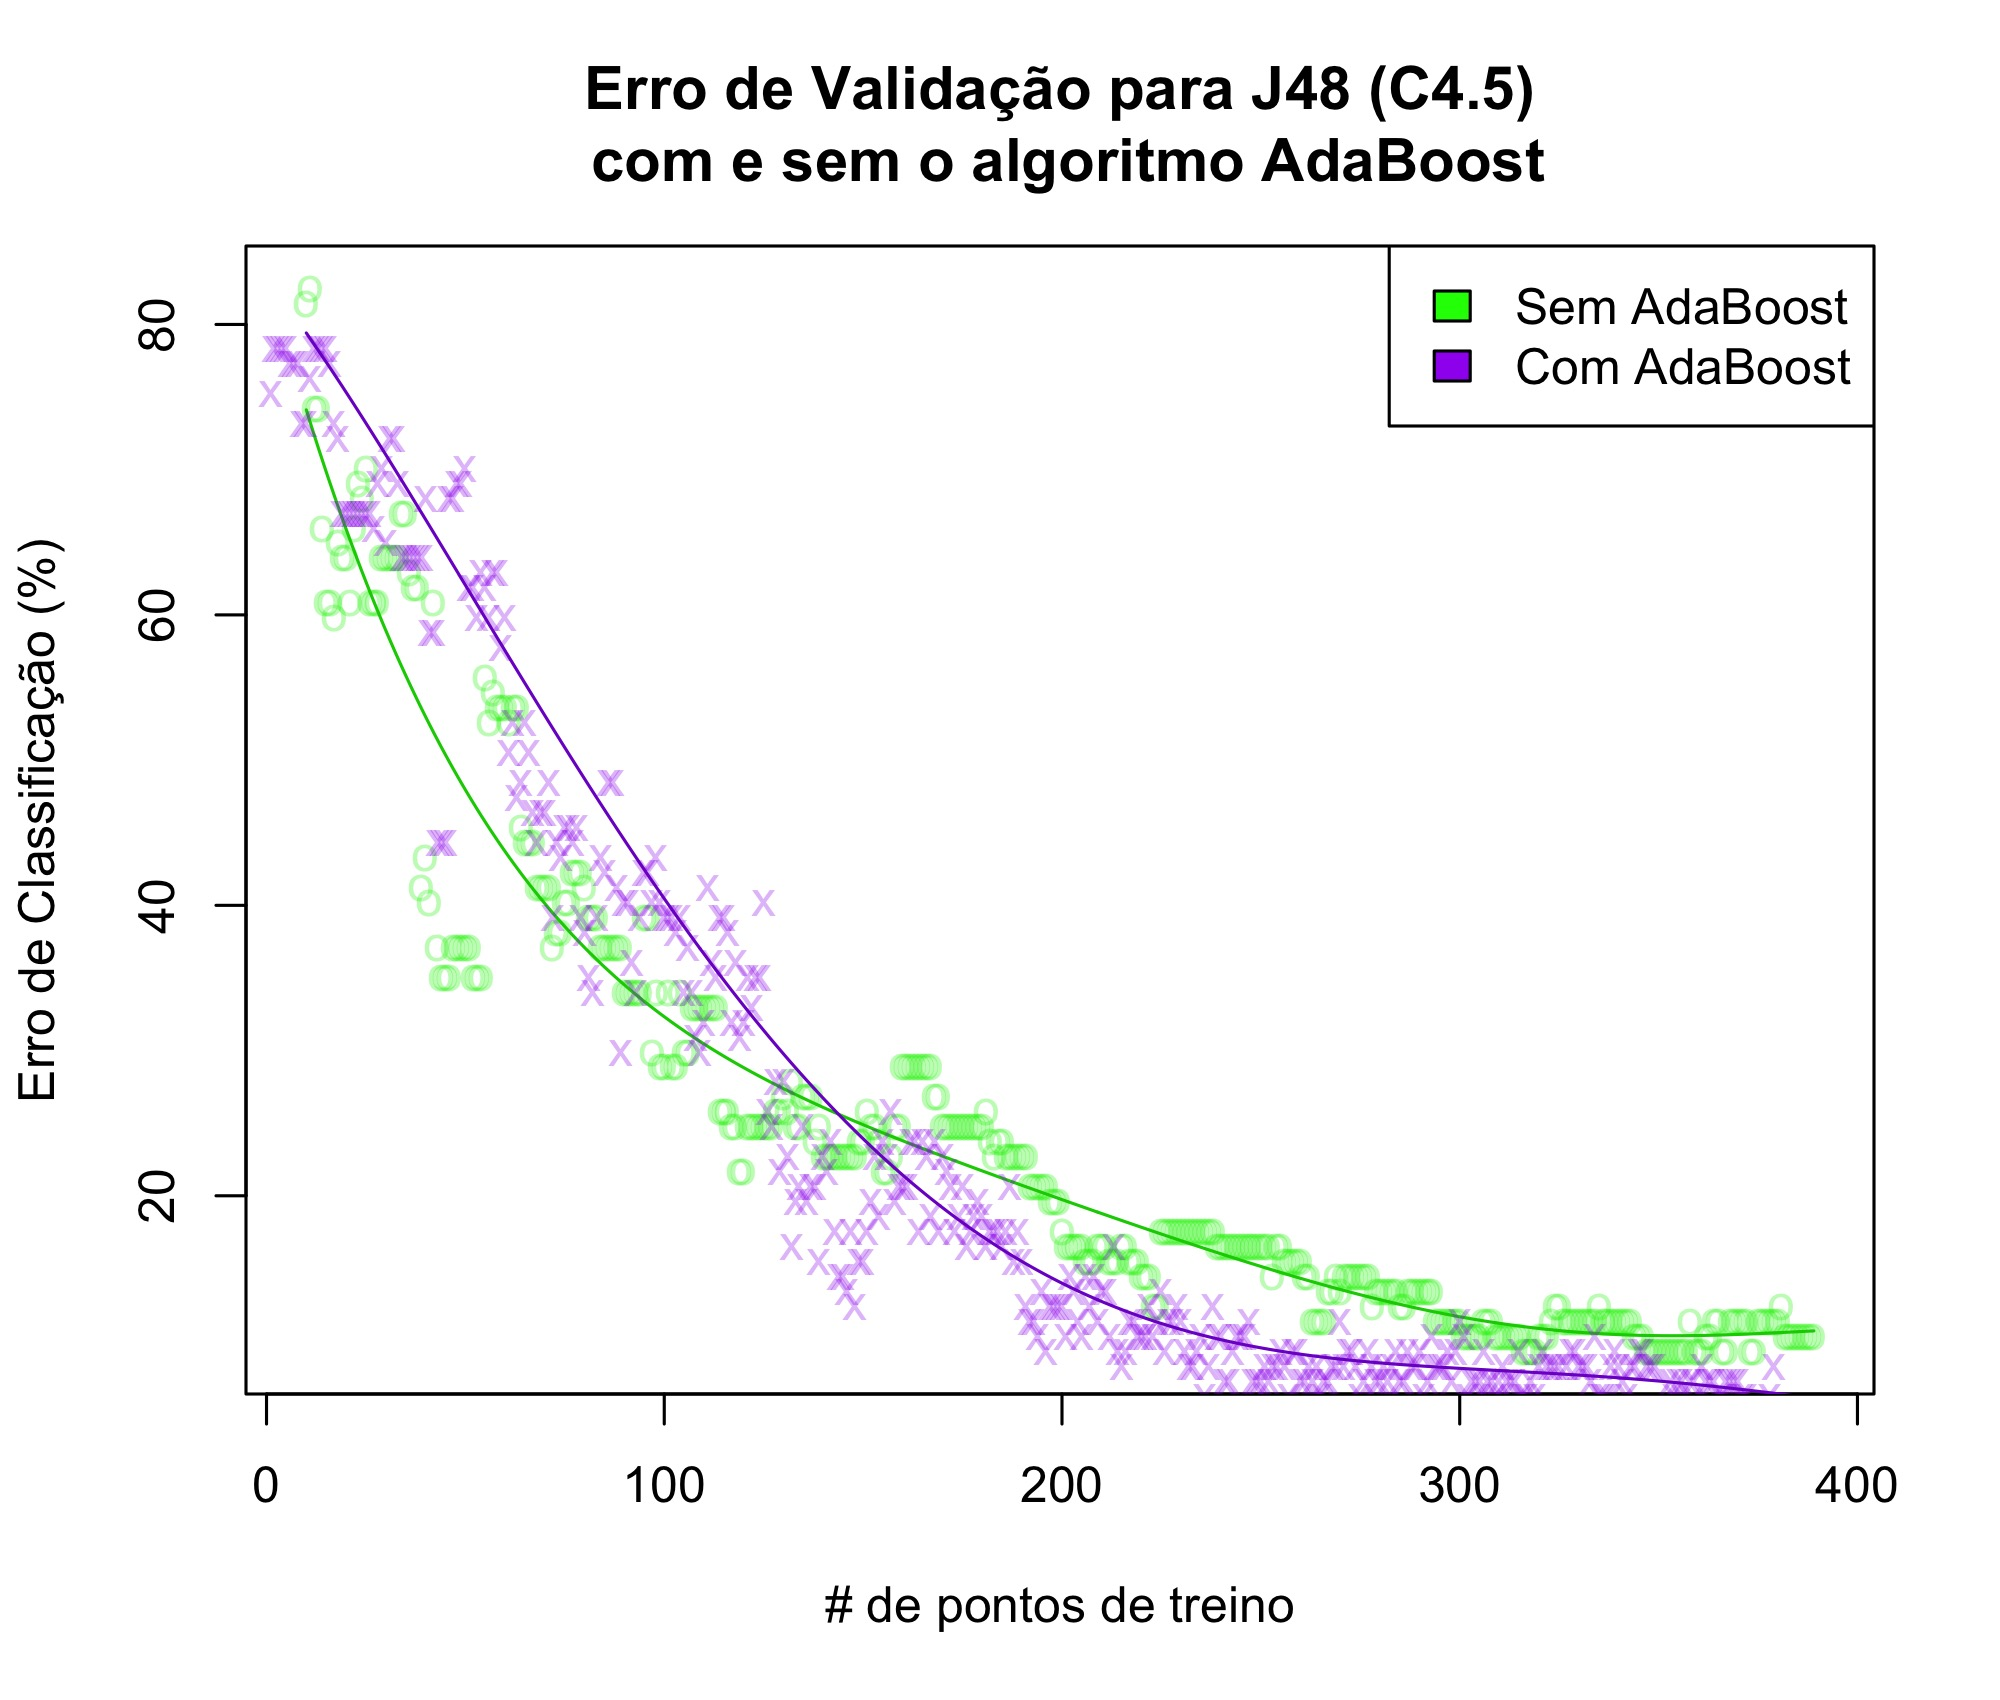
\includegraphics[width=0.9\textwidth]{J48xADAValidacaopredio1andar0}
\label{fig:comparisonC4.5andAdaBoost}  
\end{figure}


Podemos notar que com um número grande de pontos de treino, obtemos uma melhora sensível de precisão para a classificação, e portanto, no restante do trabalho, iremos usar o algoritmo C4.5 acoplado com o algoritmo AdaBoost.



\subsection{Comparação dos Modelos Usados}


Reiterando o que foi explicado em outra sessão, os testes a seguir irão contemplar todos os modelos usados. Os modelos tem seu erro testado para \textit{datasets} com um número crescente de zonas aleatórias a serem classificadas. Todos os testes foram feitos com os dados do primeiro andar do prédio 1 do \textit{dataset UJIIndoorLoc }(i.e. BuildingID 1, FloorID 0).


\begin{figure}
	\centering
	\caption{Erro do algoritmo SMO  para uma quantidade crescente de zonas de classificação.}
  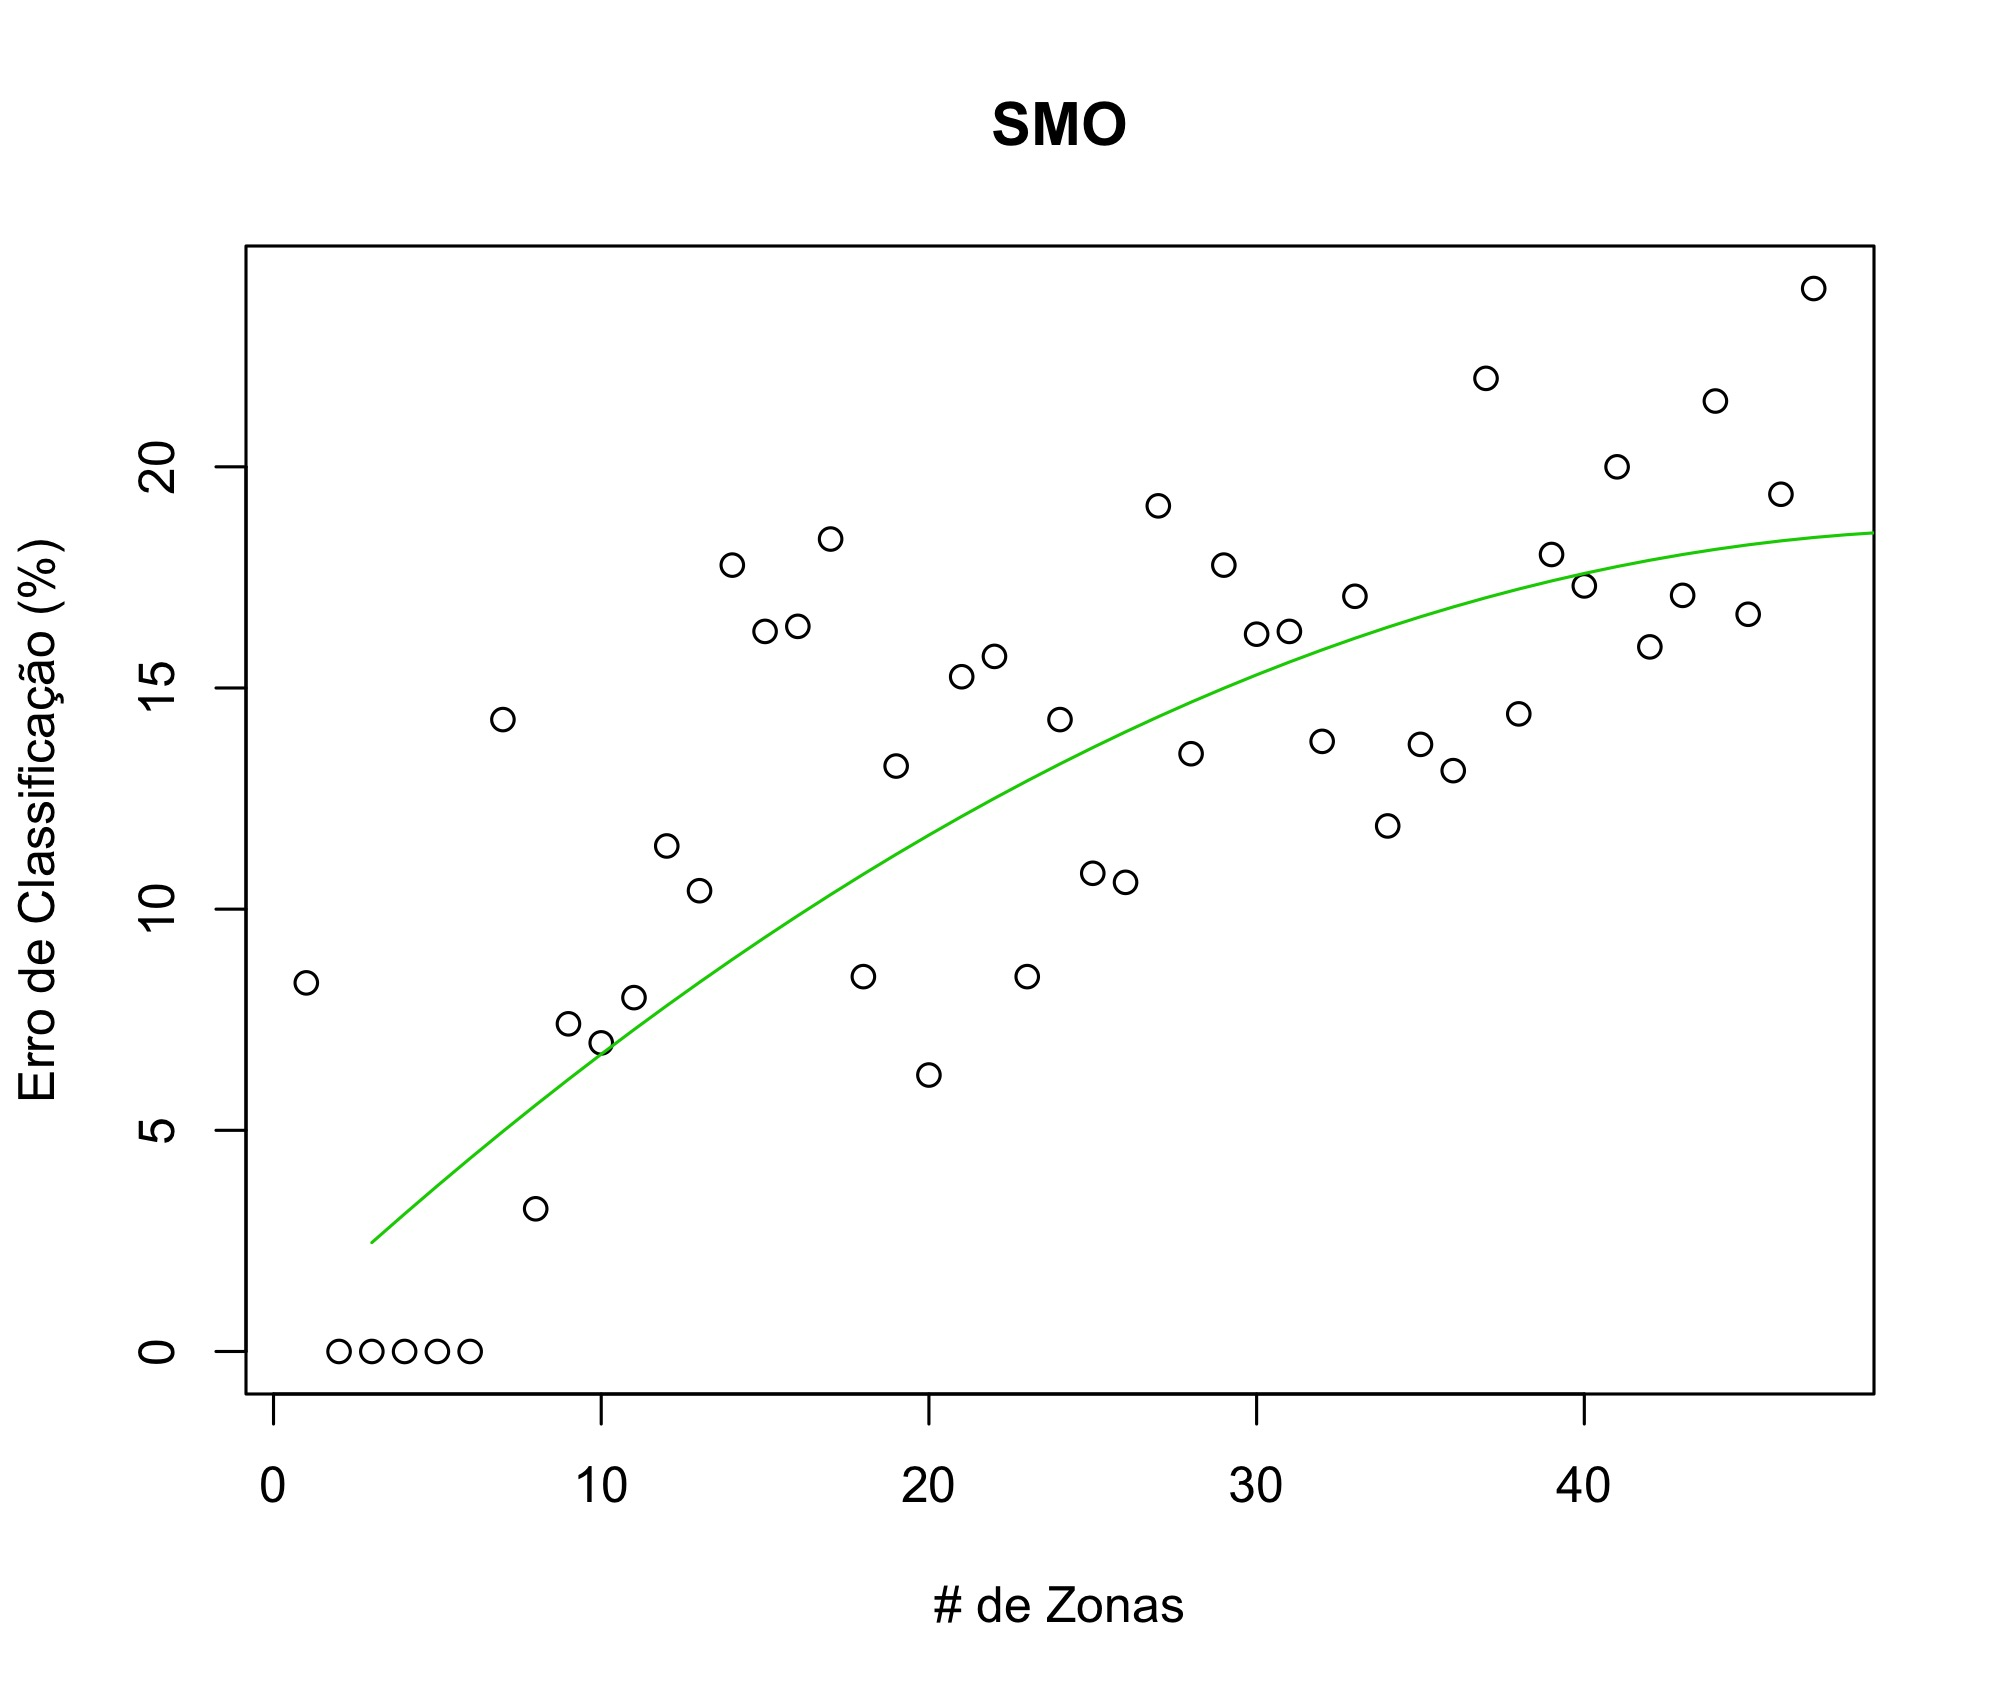
\includegraphics[width=0.8\textwidth]{errorporzonaSMO}
\label{fig:zonaSMO}

\end{figure}



\begin{figure}
	\centering
	\caption{Erro do algoritmo de Redes Neurais  para uma quantidade crescente de zonas de classificação.}
  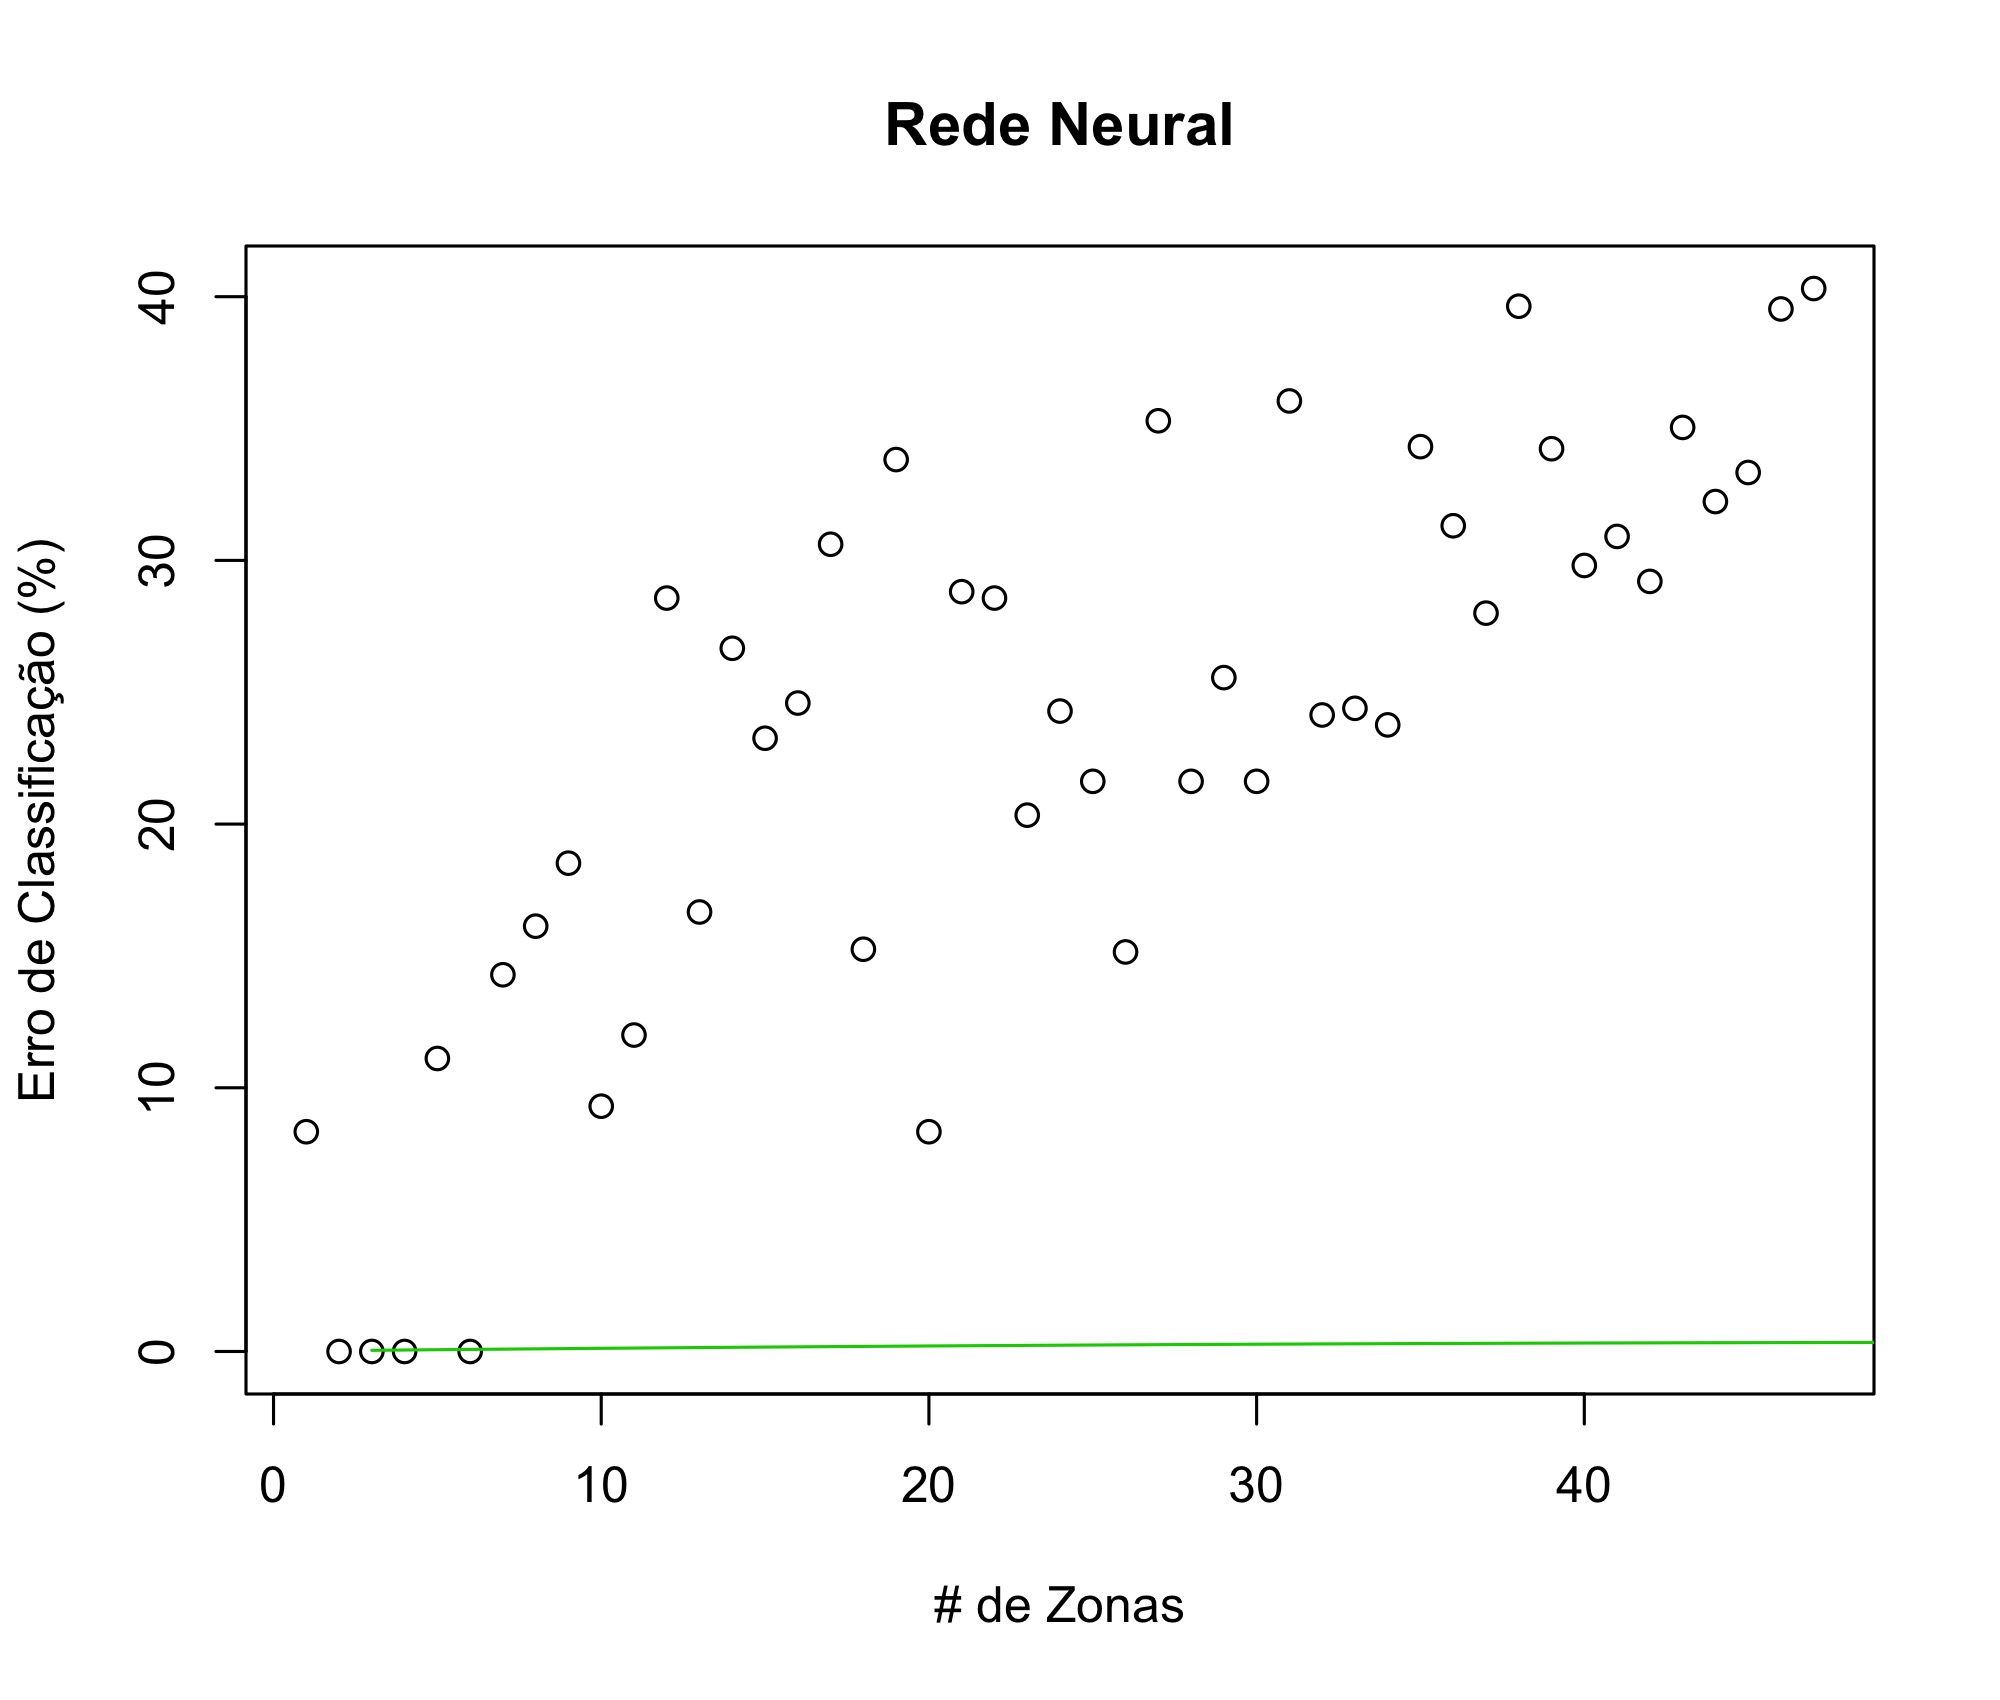
\includegraphics[width=0.8\textwidth]{errorporzonaNN}
\label{fig:zonaNN}

\end{figure}


\begin{figure}
	\centering
	\caption{Erro do algoritmo KNN para uma quantidade crescente de zonas de classificação.}
  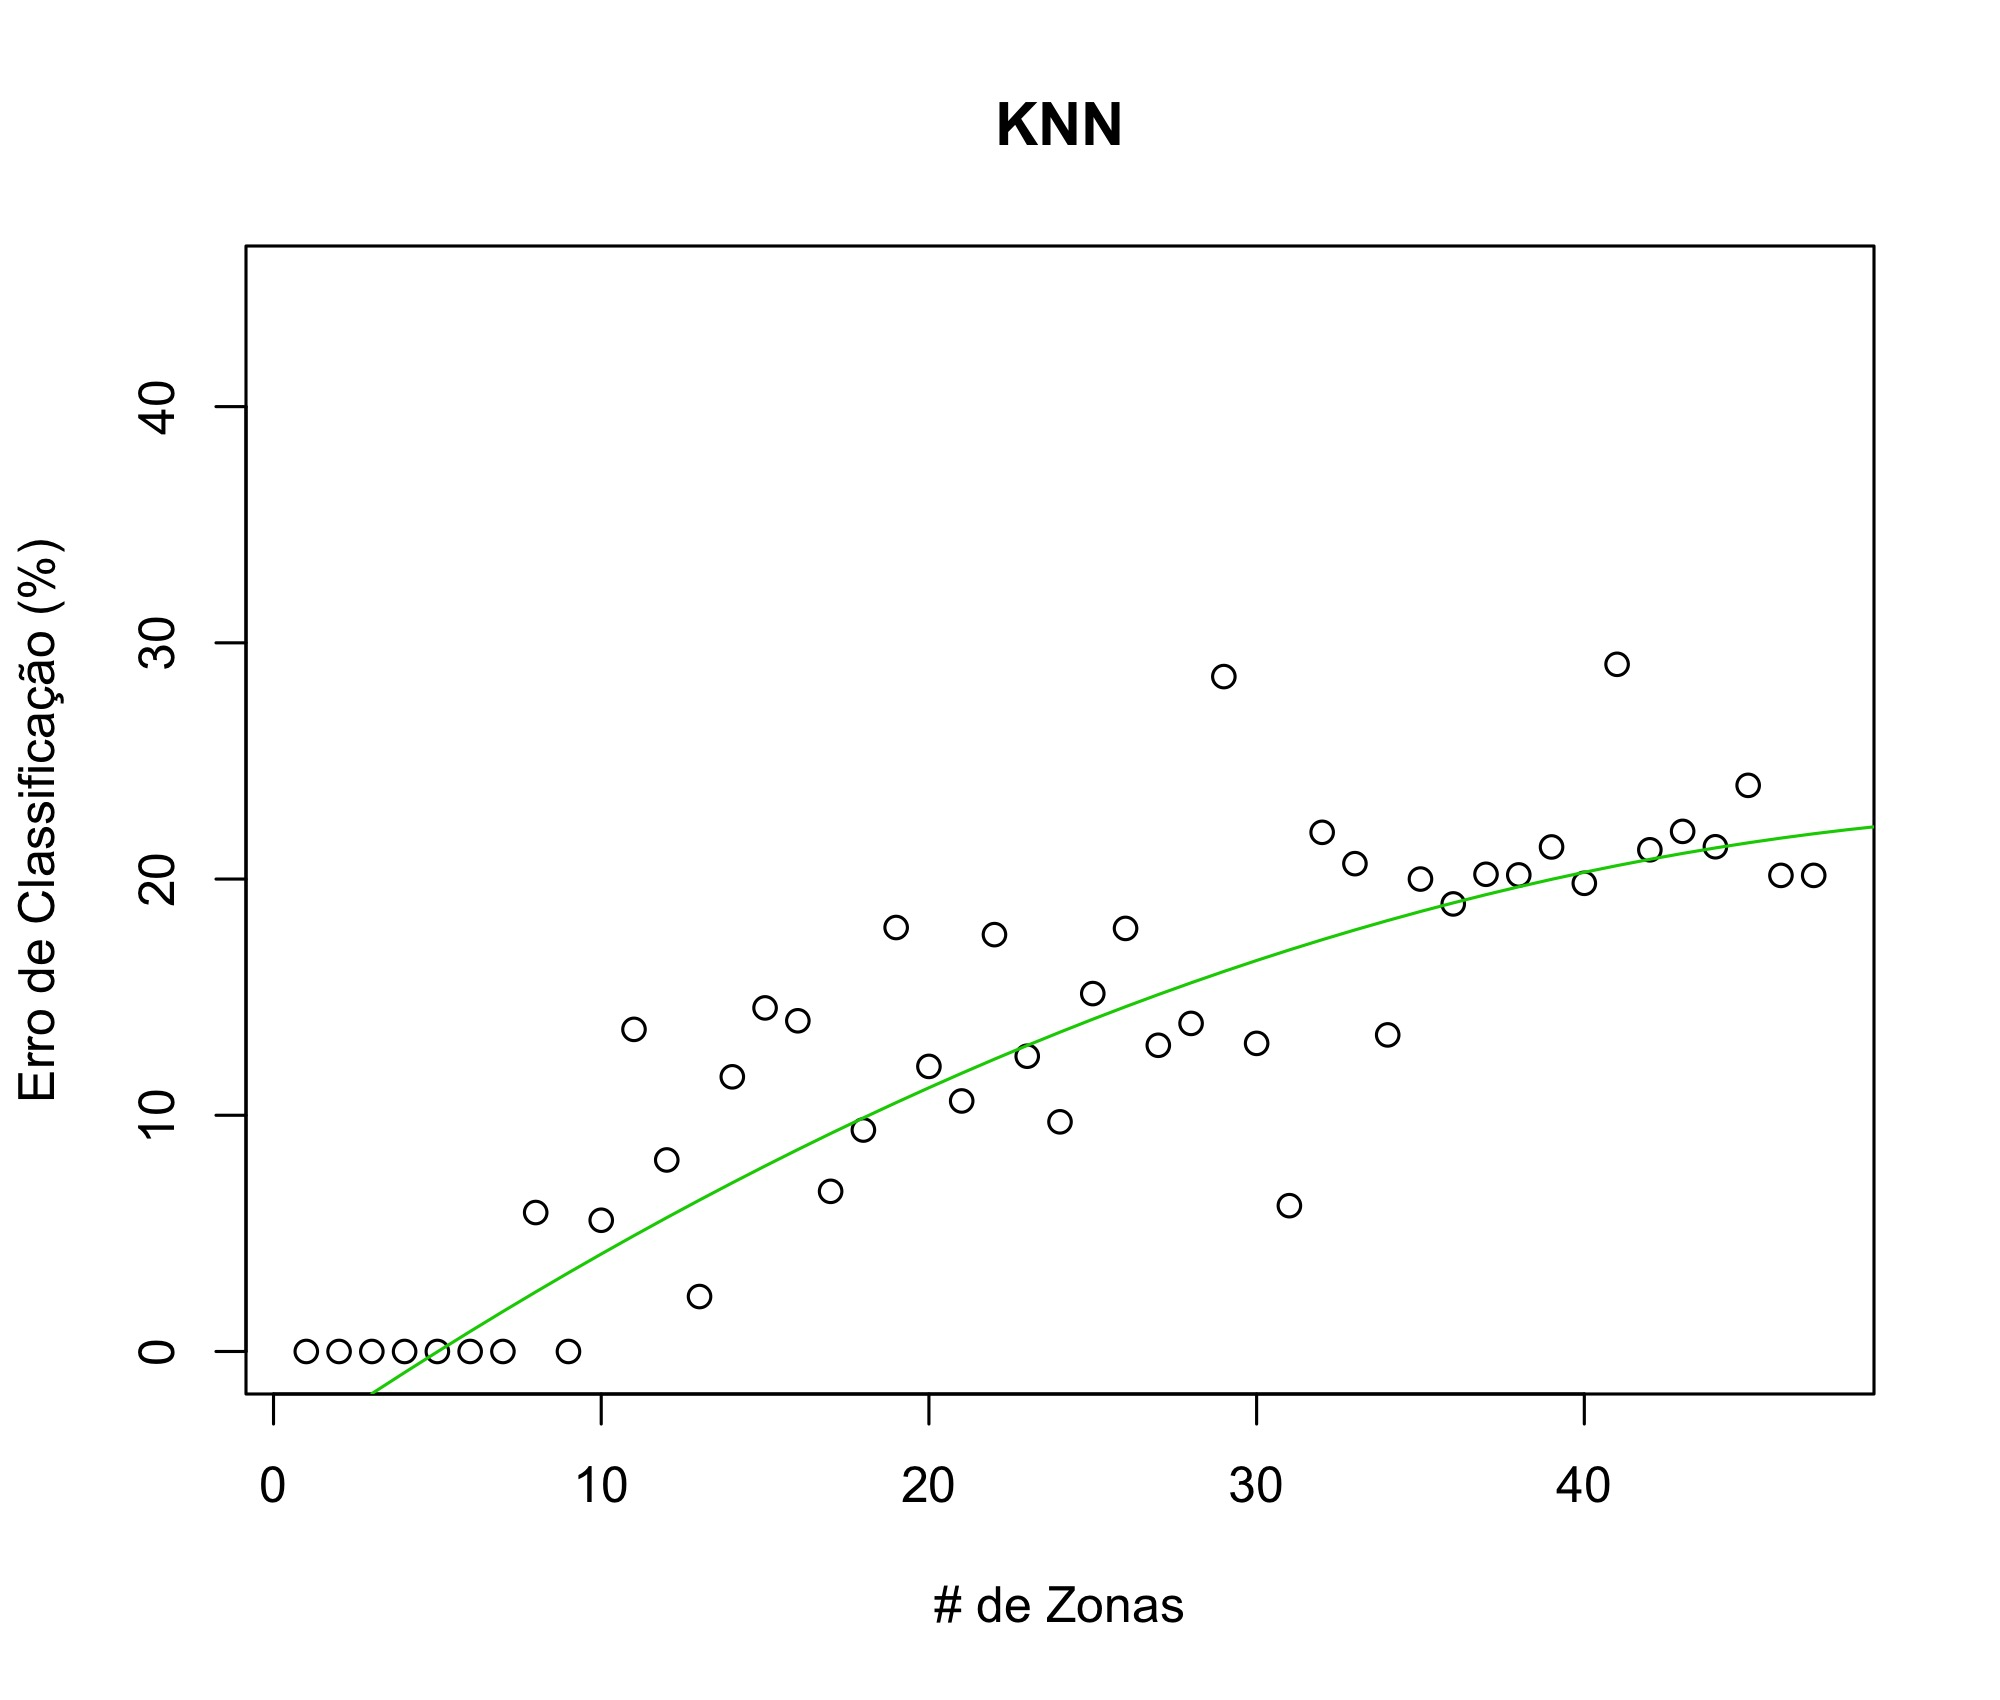
\includegraphics[width=0.8\textwidth]{errorporzonaKNN}
\label{fig:zonaKNN}

\end{figure}



\begin{figure}
	\centering
	\caption{Erro do algoritmo de Árvore de Decisão com e sem o Adaboost  para uma quantidade crescente de zonas de classificação.}
  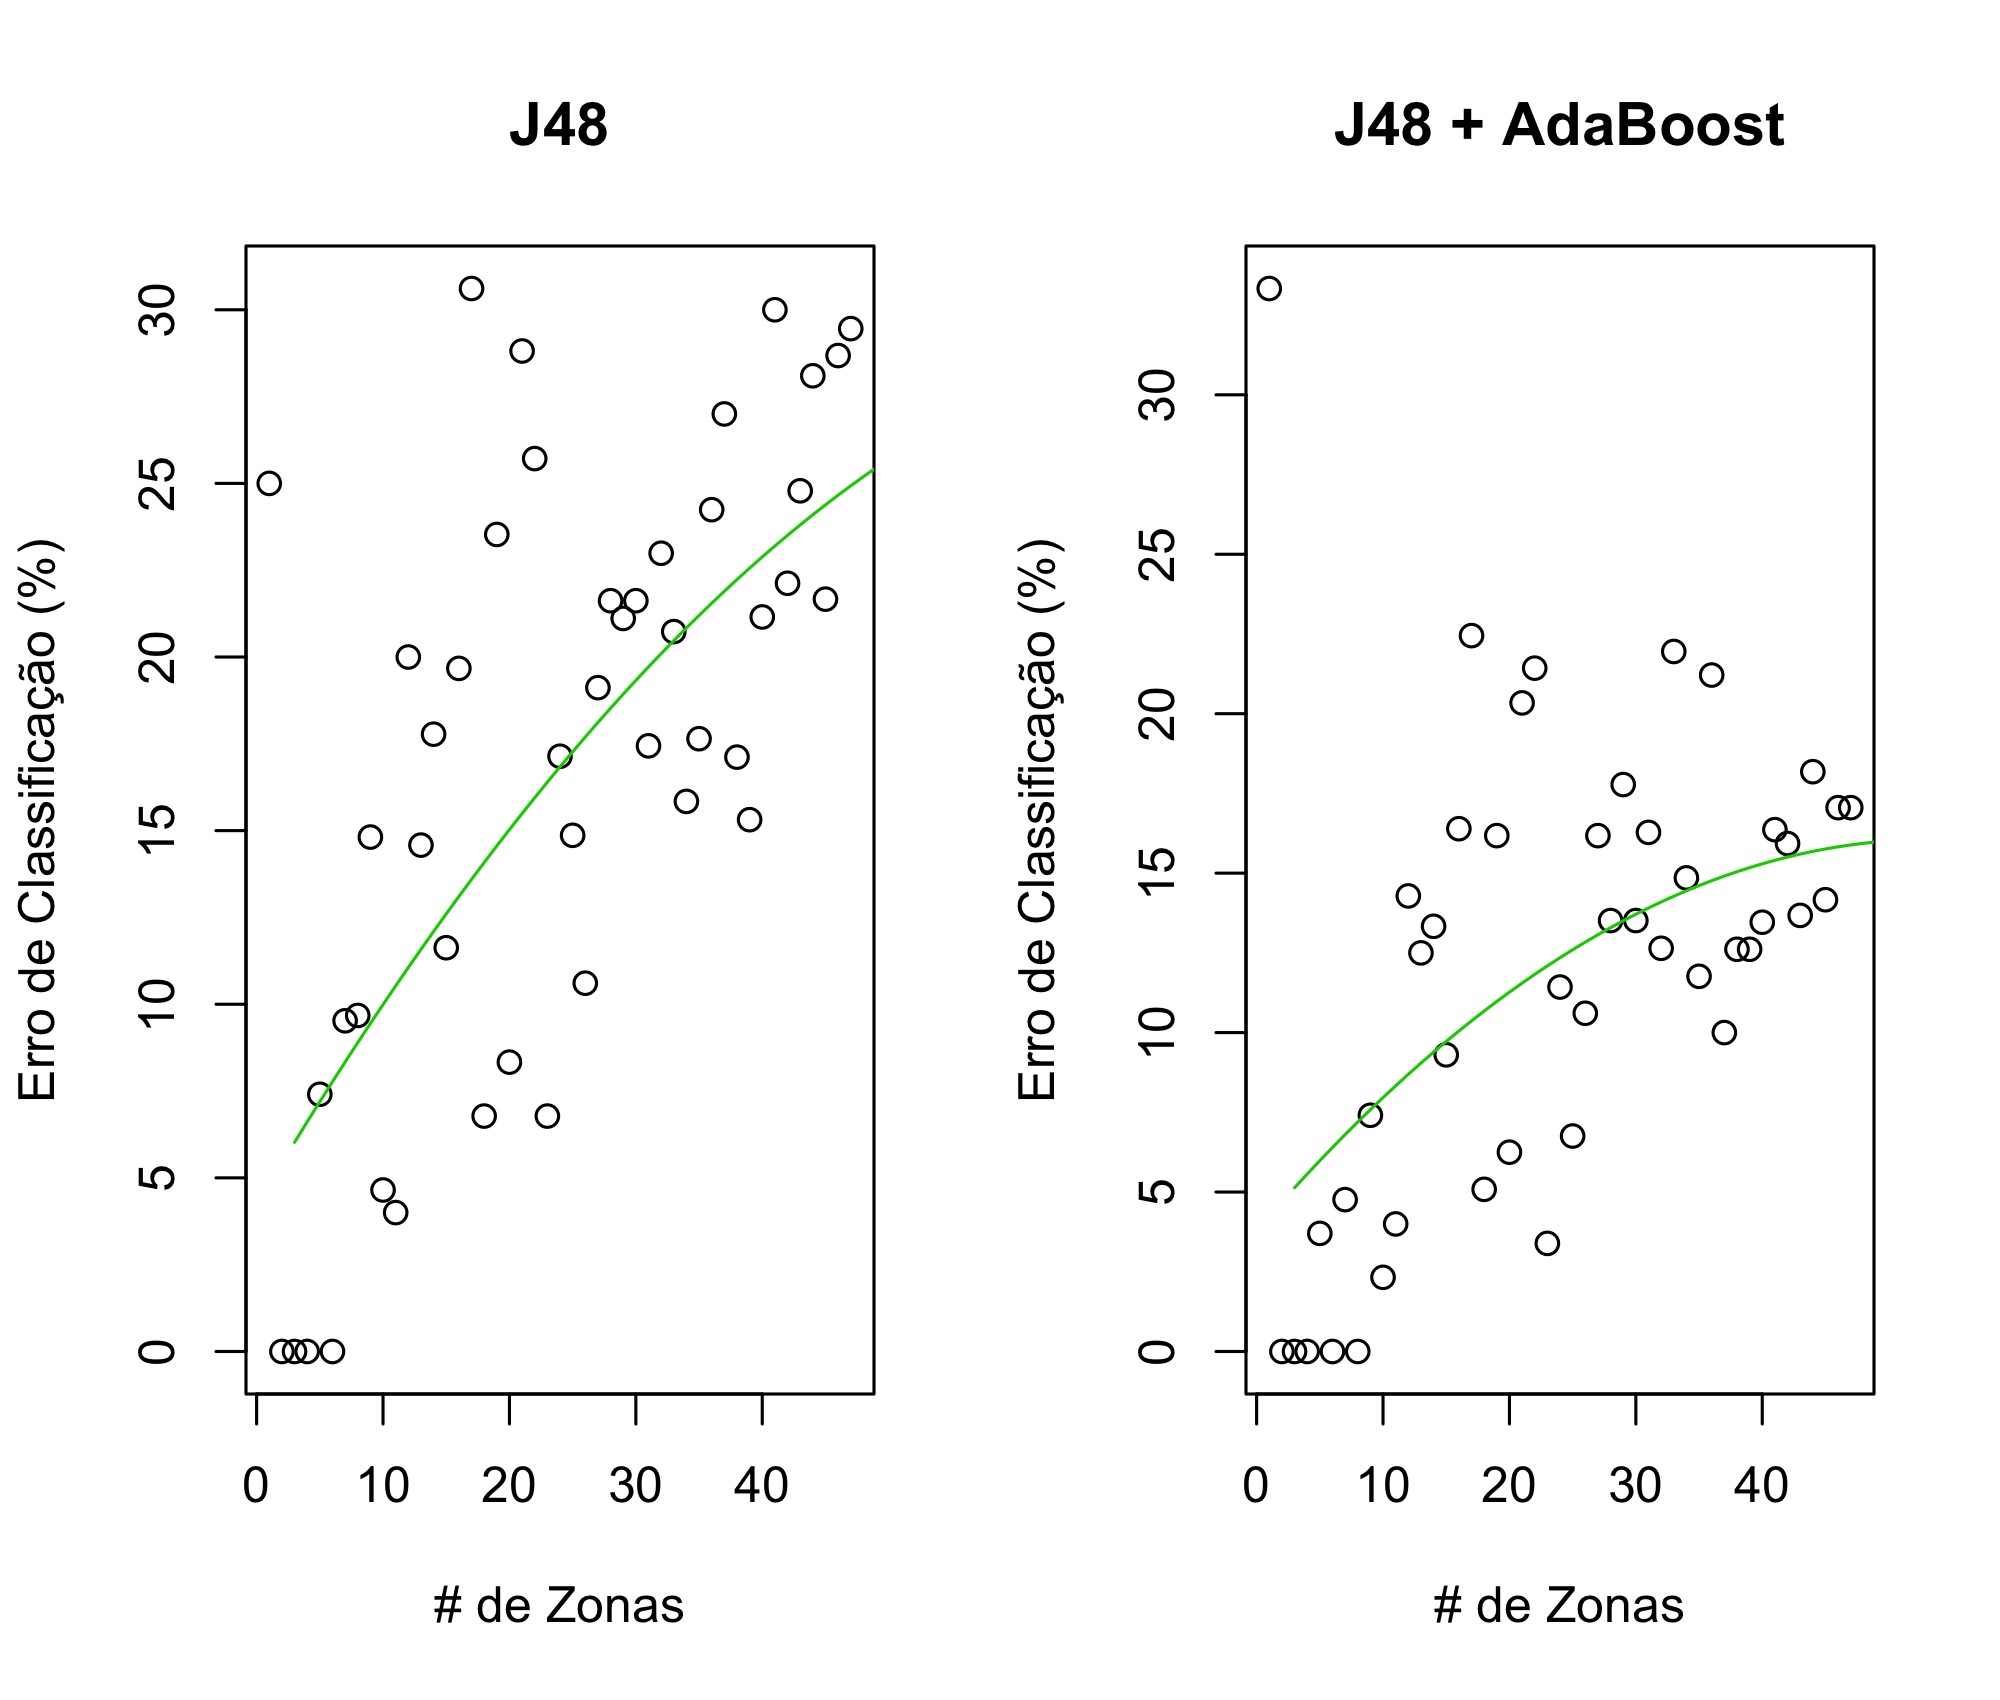
\includegraphics[width=0.8\textwidth]{errorporzonaJ48+Ada}
\label{fig:zonaAda}

\end{figure}

\clearpage


\section{Métodos de Votação}

Os chamados sistemas de \textit{Ensemble Learning} são aqueles em que uma classificação é feita com base em diversos modelos treinados. Em tópicos anteriores foi discutido o uso do algoritmo AdaBoost, que é um método desse tipo para melhorar o poder de classificadores fracos treinando iterativamente diversos modelos fracos progressivamente com os erros do anterior \cite {explainingadaboost}. Porém, para agregar os modelos usados até agora, iremos implementar algo mais simples, porém seguindo a mesma lógica: Sistemas de Votação. Baseados em \cite{Nagi2013}, usaremos diversos métodos para combinar as classificações dos nossos modelos treinados. Em um, foi usado apenas a classe de saída dos modelos, e posteriormente, as probabilidades (\textit{supports}) para cada uma das classes, que também são saídas dos modelos. Esses \textit{supports} podem ser, dependendo do modelo, a probabilidade posterior ou o grau de confiança fornecido pelos algoritmos. Por exemplo, nas redes neurais a saída de um neurônio é a função sigmoide aplicada nas entradas multiplicada pela matriz de pesos da rede, que, por definição, é um número entre 0 e 1 que representa uma probabilidade.




\subsection{Testes com os Métodos de Votação}

Como na sessão de comparação dos modelos, os métodos tem seu erro testado para datasets com um número crescente de zonas aleatórias a serem classificadas. Todos os testes foram feitos com os dados do primeiro andar do prédio 1 do dataset \textit{UJIIndoorLoc} (i.e. BuildingID 1, FloorID 0).




\begin{figure}[!ht]
	\centering
	\caption{Erro do Voto Simples e Voto Ponderado para uma quantidade crescente de zonas de classificação.}
  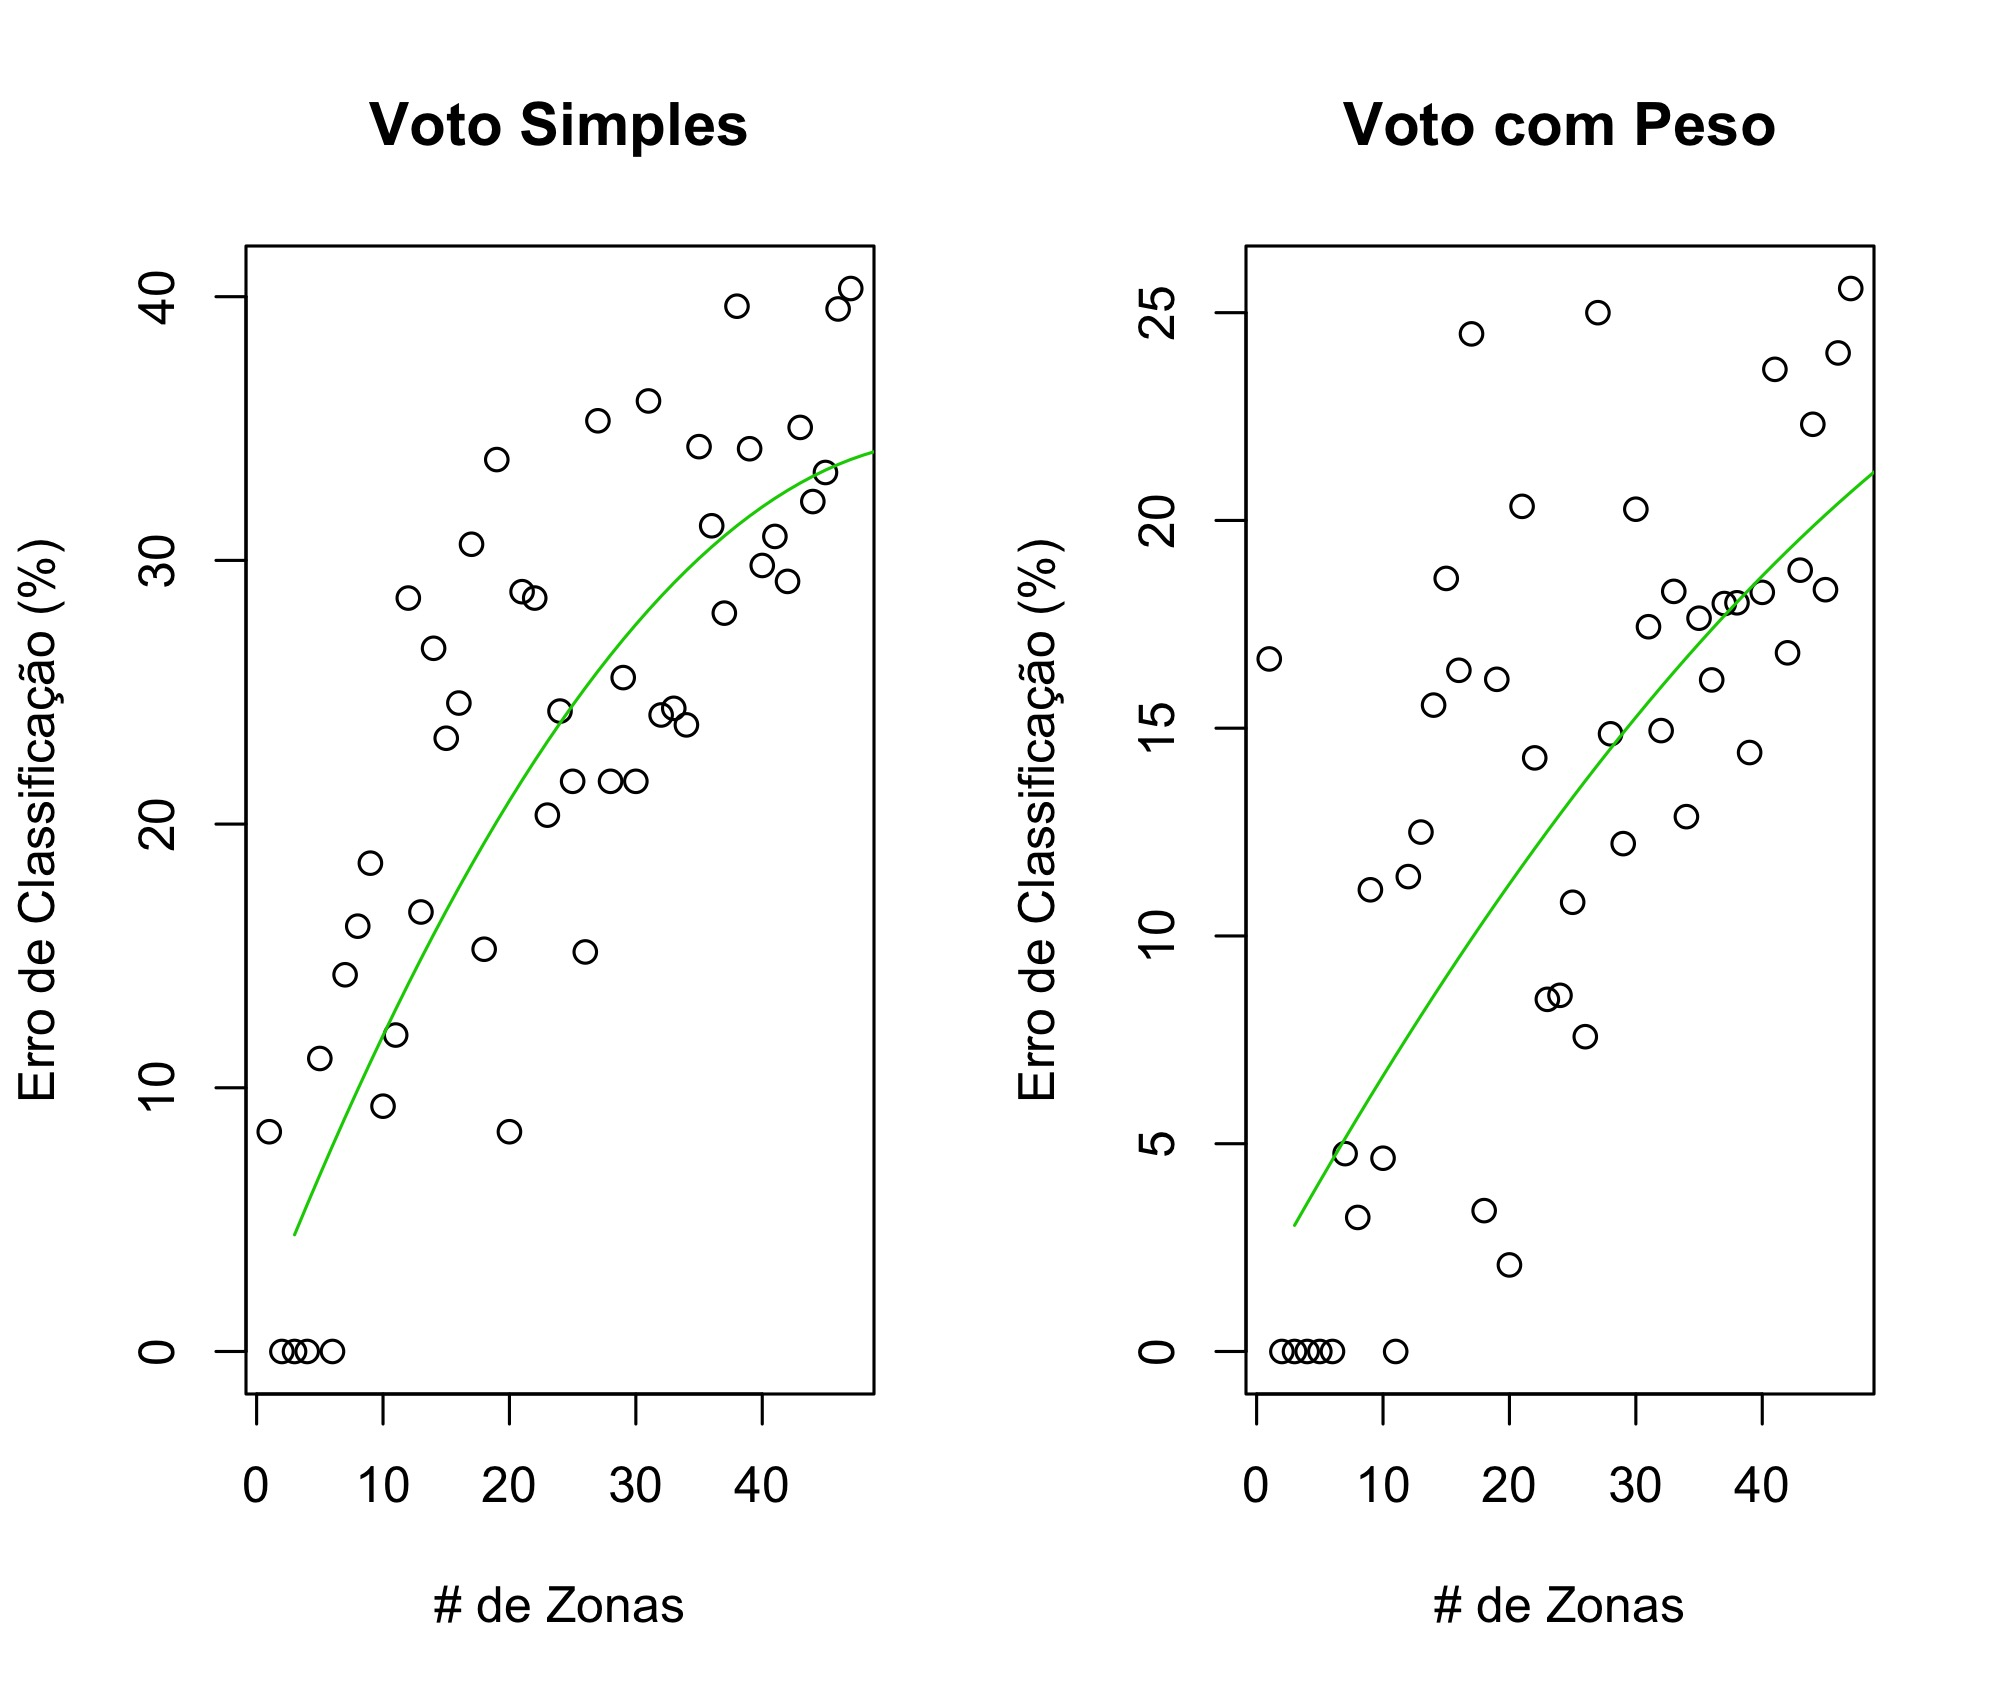
\includegraphics[width=0.9\textwidth]{errorporzonaVotos}
\label{fig:zonaVotos}

\end{figure}
